\documentclass[11pt,a4paper]{article}

\usepackage{iftex}
\ifPDFTeX
  \pdfoutput=1
  \usepackage[utf8]{inputenc}
  \usepackage[T1]{fontenc}
\fi
\usepackage[margin=1in]{geometry}
\usepackage{amsmath,amssymb,amsfonts,amsthm}
\usepackage{booktabs}
\usepackage{graphicx}
\usepackage{hyperref}
\usepackage{microtype}
\usepackage{xcolor}
\usepackage{subcaption}
\usepackage{multirow}
\usepackage{natbib}

% Toggle \anonymoustrue for double-blind ACL ARR / EMNLP / COLM peer review;
% Toggle \anonymousfalse for arXiv / TACL / public camera-ready preprint.
\newif\ifanonymous
\ifdefined\BUILDANONYMOUS
  \anonymoustrue
\else
  \anonymousfalse
\fi

\hypersetup{
    colorlinks=true,
    linkcolor=blue!60!black,
    citecolor=blue!60!black,
    urlcolor=blue!60!black
}
\emergencystretch=1.5em

\newtheorem{proposition}{Proposition}
\newtheorem{definition}{Definition}

\title{\textbf{What Earns a Phrase Its Own Token?\\Mechanistic Multi-Word Vocabulary Allocation, Compositional-Residual Folding, and Test-Time Compute Gearshifting}}

\ifanonymous
\author{
  Anonymous Authors \\
  Paper under double-blind review \\
  \small\texttt{Anonymized code \& SHA256-pinned splits included in supplementary}
}
\else
\author{
  \textbf{Andrew Rober Fouad Samy} \\
  BytesGlue \\
  \small\href{mailto:andrew.rober@bytesglue.com}{\texttt{andrew.rober@bytesglue.com}} \quad$\cdot$\quad \href{https://github.com/AndrewRober}{\texttt{github.com/AndrewRober}} \quad$\cdot$\quad \href{https://www.linkedin.com/in/andrew-rober/}{\texttt{linkedin.com/in/andrew-rober}}
}
\fi

\date{November 2026}

\begin{document}
\maketitle

\begin{abstract}
Relaxing whitespace pre-tokenization boundaries enables language model tokenizers such as SuperBPE and SupraTok to merge multi-word phrases into single tokens, reducing sequence lengths by $6\%$--$33\%$. Yet recent evaluations reveal persistent failure modes in frequency-driven superword tokenizers: severe regressions on exact next-word prediction, degraded syntactic sensitivity, and wasted vocabulary capacity from shadowed intermediate merges. We conduct a controlled 34-model empirical and mechanistic pretraining study ($30.4\text{M}$ parameters across multiple seeds and $300\text{M}$ unique tokens, scaling zero-shot to $149.6\text{M}$ parameters on deduplicated \textsc{FineWeb-Edu}) holding total vocabulary size ($V=16{,}384$), shared base subwords ($14{,}336$), deterministic segmentation, document order, and post-\citet{schaeffer2026myths} bias-corrected evaluation strictly constant.

First, we show that iterative cross-whitespace BPE wastes $33.3\%$--$37.2\%$ of superword slots on dead stepping-stone merges, and that neural pilot signals---causal continuation loss reduction (\textsc{SpilloverMerge}), cross-split Ward gradient interference (\textsc{ConflictMerge}), and counterfactual contrast margins (\textsc{ContrastMerge})---all outperform frequency (\textsc{FreqMerge}), gradient-norm selection (\textsc{VEGAD}), and \textsc{SuperBPE} under equal raw-text exposure. Second, we formalize two structural pathologies shared by existing multi-word tokenizers: \emph{Superword Vote-Splitting} (fracturing probability mass across phrase continuations sharing an initial word) and \emph{Acausal Complement Corruption} (where one-hot cross-entropy repels constituent subword embeddings from phrases sharing their prefix). We cure both with \emph{zero deployment overhead} via \textbf{Prefix-Cone Vote Aggregation} (recovering $+0.80\%$--$+1.59\%$ exact next-word accuracy with zero retraining while leaving subword controls identically unchanged) and \textbf{Foldable Compositional-Residual Parameterization} ($W_P = \frac{1}{|P|}\sum_{t\in P} W_t + \Delta_P$, folding with exact $0.0$ floating-point error into a standard embedding table, achieving the best out-of-domain generalization across all $18$ Stage~B/D models, and unsupervisedly separating opaque English idioms from transparent compounds). Third, we introduce \textbf{Attention-Query De-Multiplexing} ($D_{\text{bind}}$, vetoing multi-binding relational spans whose constituents attend to distinct upstream antecedents) and \textbf{Compute Gearshifting} (dual-granularity pretraining enabling Chain-of-Thought-free test-time accuracy scaling via input unmerging). Under equal compute (\textsc{Iso-FLOPs}), our synthesis beats both \textsc{Byte-BPE} and \textsc{SuperBPE} across every metric while cutting Layer-2 lexical stitching attention by $51.2\%$. Across $3$-seed $300\text{M}$-token confirmations and $5\times$ ($149.6\text{M}$) zero-shot vocabulary transfer, our method achieves the highest syntactic accuracy of all $34$ models ($86.44\%, p=0.0137$ at $30\text{M}$; $86.81\%$ at $150\text{M}$), top zero-shot \textsc{ARC-Easy} reasoning ($39.20\%$), complete perturbation immunity, and a $+1.58\%$ single-checkpoint test-time gearshift gain.
\end{abstract}

\section{Introduction}
Standard subword tokenizers---including Byte-Pair Encoding \citep{sennrich2016neural} and Unigram LM \citep{kudo2018subword}---enforce rigid regular-expression pre-tokenization walls at whitespace boundaries. Recently, \textsc{SuperBPE} \citep{liu2025superbpe}, \textsc{BoundlessBPE} \citep{schmidt2025boundless}, and \textsc{SupraTok} \citep{tanase2026supratok} demonstrated that permitting merges across whitespace yields substantial sequence-length compression. Unlike architectural modifications that sum modifier embeddings \citep{reif2025cobpe} or retain massive auxiliary $n$-gram embedding tables at inference \citep{huang2025overtokenized}, a static vocabulary mixing subwords and multi-word phrases requires \emph{zero changes} to production Transformer serving runtimes (\texttt{vLLM}, \texttt{TensorRT-LLM}, \texttt{llama.cpp}).

However, treating cross-whitespace vocabulary construction purely as string compression leaves three core scientific problems unresolved:
\begin{enumerate}
    \item \textbf{Confounded Attribution:} Prior studies alter base vocabularies, curriculum schedules, intermediate merge trees, and effective byte context windows simultaneously, obscuring \emph{why} a multi-word span earns its own dedicated vector in a Transformer.
    \item \textbf{Unexplained Accuracy Collapses:} Follow-up benchmarks document sharp regressions in \textsc{SuperBPE} on exact word-prediction benchmarks and fine-grained syntactic minimal pairs, without a formal mechanistic diagnosis or inference fix.
    \item \textbf{Evaluation Pitfalls:} \citet{schaeffer2026myths} recently proved that raw Bits-Per-Byte (BPB) favors higher-compression vocabularies even on uniform random weights ($\text{BPB}_{\text{init}} = (\text{tokens}/\text{byte}) \cdot \log_2 V$), while standard \textsc{BLiMP} minimal pairs \citep{warstadt2020blimp} are confounded whenever grammatical and ungrammatical sentences tokenize to unequal lengths.
\end{enumerate}

In this paper, we recast multi-word tokenization mechanistically: \emph{inside an autoregressive Transformer, sequence positions are serial clock ticks of multi-head attention and MLP computation, whereas vocabulary rows act as $O(1)$ non-linear lookup memory.} Allocating a vocabulary slot to a multi-word phrase $P=(t_1,\dots,t_k)$ trades $k-1$ sequential residual-stream updates for a table lookup. That trade helps when $P$ is a compositionally opaque lexical unit or polysemous collocation whose constituents pull optimization in conflicting directions, and \emph{hurts} when $P$ is a multi-binding relational span (e.g., \texttt{"he told her"}) where collapsing $k$ positions creates an attention-query bottleneck, or when greedy lookahead segmentation starves base words of training signal and splits output probability mass.

\paragraph{Summary of Contributions.}
\begin{itemize}
    \item \textbf{Controlled 11-Method Benchmark \& Slot-Waste Audit (Sections~\ref{sec:framework}--\ref{sec:stage_b}):} Fixing a shared $14{,}336$-token lossless Byte-BPE base and $2{,}048$ phrase slots ($V=16{,}384$), we compare five published baselines (\textsc{Byte-BPE}, \textsc{Unigram}, \textsc{SaGe}, \textsc{SuperBPE}, \textsc{SupraTok}), a shared-machinery frequency null control (\textsc{FreqMerge}), \textsc{VEGAD} gradient-magnitude control \citep{liu2024gold}, and five mechanistic selection hypotheses. We show iterative merging in \textsc{SuperBPE} and \textsc{SupraTok} leaves $37.2\%$ and $33.3\%$ of phrase slots unemitted on held-out text, whereas direct boundary-guarded allocation achieves $95.2\%$--$99.0\%$ active slot utilization.
    \item \textbf{Curing Vote-Splitting \& Acausal Complement Corruption (Section~\ref{sec:vote_fold}):} We prove how acausal lookahead segmentation causes \emph{Superword Vote-Splitting} at decoding time and \emph{Swiss-Cheese Complement Embeddings} during training. We introduce \textbf{Prefix-Cone Vote Aggregation} (yielding up to $+1.59\%$ exact next-word recovery with zero retraining and exact $0.00\%$ invariance on subword models) and \textbf{Foldable Compositional-Residual Parameterization}, which achieves the \#1 out-of-domain \textsc{TinyStories} BPB ($1.41790$) of all $18$ Stage~B/D models, folds with exact $0.0$ floating-point error into an unmodified Transformer, and unsupervisedly discovers English idioms via $\|\Delta_P\|_2$.
    \item \textbf{Attention-Query De-Multiplexing, Compute Gearshifting, \& $5\times$ Zero-Shot Scale-Up (Sections~\ref{sec:demux_gear}--\ref{sec:scaleup}):} Vetoing multi-binding relational spans via cross-constituent prefix attention divergence ($D_{\text{bind}}$) and training with $20\%$ dual-granularity unmerging (\textsc{BT3}) beats both \textsc{Byte-BPE} and \textsc{SuperBPE} across every metric at equal compute (\textsc{Iso-FLOPs}), cuts Layer-2 previous-token stitching by $51.2\%$, confirms statistical significance across $3$ paired seeds at $300\text{M}$ unique tokens ($p=0.0137$), and transfers zero-shot to $149.6\text{M}$ parameters ($5\times$ scale), winning \textsc{BLiMP} ($86.81\%$) and \textsc{ARC-Easy} ($39.20\%$) while scaling single-checkpoint accuracy by $+1.58\%$ at test time.
\end{itemize}

\section{Related Work}
\label{sec:related}
\paragraph{Subword and Context-Aware Tokenization.}
Classical subword algorithms construct vocabularies via greedy byte/character pair frequency \citep{sennrich2016neural} or unigram marginal likelihood pruning \citep{kudo2018subword}. Context-aware subword pruning methods such as \textsc{SaGe} \citep{yehezkel2023incorporating} replace unigram likelihood with SkipGram ablation losses within single words, while \textsc{LiteToken} \citep{yang2026litetoken} removes unreachable intra-word BPE merge residues. Domain-adaptation methods such as \textsc{VEGAD} \citep{liu2024gold} score candidate domain tokens using input gradient norms. We include \textsc{Byte-BPE}, \textsc{Unigram}, \textsc{SaGe}, and \textsc{VEGAD} as controlled baselines, showing that directional cross-split Ward gradient conflict (\textsc{C1}) and causal continuation spillover (\textsc{C3}) outperform raw gradient magnitude.

\paragraph{Cross-Boundary Superwords and $n$-Gram Representations.}
\textsc{SuperBPE} \citep{liu2025superbpe} and \textsc{BoundlessBPE} \citep{schmidt2025boundless} lift regex pre-tokenization walls late in BPE training, whereas \textsc{SupraTok} \citep{tanase2026supratok} introduces staged Pointwise Mutual Information (PMI) filtering across boundaries. Orthogonally, \textsc{CoBPE} \citep{reif2025cobpe} modifies the Transformer input layer to sum compositional modifier embeddings, and \textsc{Over-Tokenized Transformers} \citep{huang2025overtokenized} attach multi-million-row $n$-gram input tables. Unlike \textsc{CoBPE} or \textsc{Over-Tokenized}, our Foldable Compositional-Residual parameterization acts purely as a \emph{pretraining re-parameterization} that folds algebraically into a standard $[V, d]$ lookup table with zero extra parameters or runtime operations.

\paragraph{Tokenization Regularization and Marginalization.}
\textsc{BPE-Dropout} \citep{provilkov2020bpe} randomly drops merges during neural machine translation training for robustness, while \citet{cao2021bench} show that evaluating multi-segmentation models along a single canonical path understates surface string probability unless marginalized. Extending these insights, we derive the exact closed-form single-path cross-entropy split $\Delta\text{BPB}(q) = f_{\text{phrase}}(-\log_2(1-q))/B$ under dual-granularity pretraining and repurpose granularity switching at inference time as an adaptive test-time compute knob (\emph{Compute Gearshifting}) complementary to pause tokens \citep{goyal2024think}.

\section{Controlled Experimental Framework}
\label{sec:framework}

\subsection{Shared Tokenization Machinery \& Morphological Boundary Guard}
Every vocabulary in our study has exact size $V=16{,}384$, comprising two special tokens (\texttt{<|endoftext|>}, \texttt{<|pad|>}) and all $256$ byte fallback tokens, guaranteeing $100\%$ lossless UTF-8 byte round-tripping without destructive text normalization (\texttt{NFKC} and whitespace collapsing are disabled across all methods, including \textsc{Unigram} and \textsc{SaGe}). For all controlled multi-word methods (\textsc{C0}--\textsc{C5}, \textsc{VEGAD}, and \textsc{BT1}--\textsc{BT3}), we train one shared $14{,}336$-entry Byte-BPE base tokenizer strictly on training text and allocate the remaining $K=2{,}048$ slots ($12.5\%$) to multi-word spans ($2$--$4$ words, document frequency $\ge 25$).

\paragraph{Preventing Subword-Suffix Stranding.}
Naive phrase matching over base token IDs introduces a morphological bug whenever a derived word splits in the $14{,}336$ base vocabulary (e.g., \texttt{" New Yorker"} $\to$ \texttt{["\textvisiblespace New", "\textvisiblespace York", "er"]}): greedy replacement merges \texttt{("\textvisiblespace New", "\textvisiblespace York")} inside \texttt{" New Yorker"}, stranding suffix \texttt{"er"}. Our segmenter enforces a strict right-boundary guard: span $[i, j)$ matches only if $t_i$ begins at a word start and $t_j$ (if present) is not an intra-word alphanumeric continuation subword. We support both deterministic left-to-right longest match (\texttt{greedy\_ltr}) and exact $O(N)$ weighted-interval dynamic programming (\texttt{utility\_dp}).

\subsection{Five Mechanistic Candidate Selectors}
\paragraph{C0: \textsc{FreqMerge} (Shared-Machinery Null Control).} Iteratively selects $2{,}048$ phrases maximizing active token savings $\text{count}(p)\cdot(|p|-1)$ with batched corpus re-segmentation to prevent shadowed slots.

\paragraph{C1: \textsc{ConflictMerge} (Cross-Split Ward Gradient Divergence).}
Naive cosine conflict $-\cos(\bar{g}_{t,\text{in }p}, \bar{g}_{t,\text{out }p})$ suffers a hidden degeneracy in tied-embedding Transformers: near stationarity, $G_{t,\text{input}} + G_{t,\text{output}} \approx 0$, and because $N_{\text{in}} \ll N_{\text{out}}$, $\bar{g}_{t,\text{out }p} \approx -\frac{1}{N_t}G_{t,\text{output}}$, contaminating input conflict with output-logit frequency pressure. Instead, we partition calibration documents into disjoint halves $A, B$, attach hooks strictly to input-embedding activations of a $30.4\text{M}$ base pilot model, and compute the exact cross-split Ward variance reduction (first-order optimization energy freed by unsharing $p$):
\begin{equation}
    I(p) = \sum_{t \in p} \max\!\left(0, \; \frac{N_{t,\text{in}} N_{t,\text{out}}}{N_{t,\text{in}} + N_{t,\text{out}}} \left\langle \bar{g}_{t,\text{in}}^{(A)} - \bar{g}_{t,\text{out}}^{(A)}, \; \bar{g}_{t,\text{in}}^{(B)} - \bar{g}_{t,\text{out}}^{(B)} \right\rangle \right).
\end{equation}
Global token offsets cancel identically in $\bar{g}_{t,\text{in}} - \bar{g}_{t,\text{out}}$, and mini-batch noise has strictly zero cross-split expectation. We pair \textsc{C1} with \textsc{Control\_VEGAD} \citep{liu2024gold}, ranking phrases by accumulated input gradient norms $\sum \|g_{t,i}\|_2$ on the identical pilot and splits.

\paragraph{C2: \textsc{ReserveMerge} (Component-Exposure Guard).} Penalizes phrase additions that push standalone emissions of any constituent token below a healthy exposure floor, protecting reusable building blocks from ``Magikarp'' under-training \citep{land2024fishing}.

\paragraph{C3: \textsc{SpilloverMerge} (Causal Continuation Gain).} Fits L2-anchored temporary input embeddings $e_p \in \mathbb{R}^{d}$ on Calibration Split $A$ through the frozen pilot (keeping the output softmax vocabulary fixed at $14{,}336$ so partition functions cannot drift), then scores the lower confidence bound of causal negative log-likelihood reduction strictly on the \emph{subsequent} unmerged continuation on disjoint Split $B$: $S(p) = \mathbb{E}_B[\mathcal{L}_{\text{cont}}(\text{split}) - \mathcal{L}_{\text{cont}}(\text{merged})]$.

\paragraph{C4: \textsc{BoundaryStableMerge}.} Evaluates candidate batches incrementally on controlled punctuation, spacing, and character-typo snippet pairs, penalizing unchanged-region token boundary shifts.

\paragraph{C5: \textsc{ContrastMerge}.} Generates $100\%$ self-supervised counterfactual continuations directly from training occurrences (agreement flips, polarity/quantity swaps, and entity swaps), rewarding phrases whose merged representations widen the log-likelihood margin $M_{\text{merged}}(p) - M_{\text{split}}(p)$ on Split $B$.

\begin{figure}[t]
    \centering
    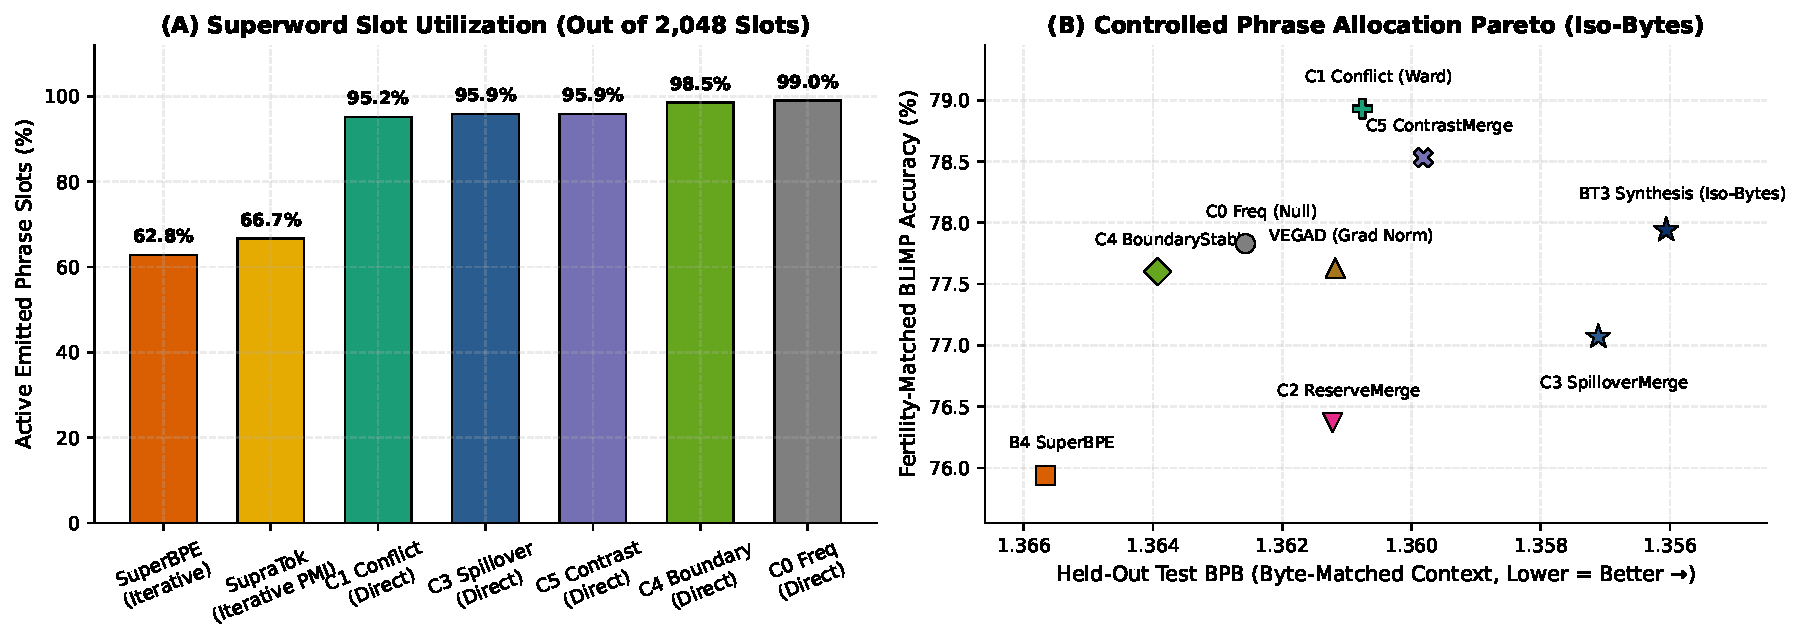
\includegraphics[width=\textwidth]{figures/fig1_slot_waste_and_stage_b.pdf}
    \caption{\textbf{(A)} Active phrase slot utilization out of $2{,}048$ superword entries on held-out validation text: iterative BPE merging (\textsc{SuperBPE}, \textsc{SupraTok}) leaves $33\%$--$37\%$ of phrase slots unemitted due to shadowed stepping-stone merges, whereas direct allocation (\textsc{C0}--\textsc{C5}) achieves $95\%$--$99\%$ utilization. \textbf{(B)} Controlled Iso-Bytes Pareto frontier across shared-foundation multi-word selectors ($V=16{,}384$, $30.42\text{M}$ parameters).}
    \label{fig:stage_b}
\end{figure}

\subsection{Architectures, Training Regimes, \& Bias-Corrected Evaluation}
All Stage B/C/D models use an identical bias-free Decoder Transformer ($7$ blocks, $d=512$, $8$ heads, $d_{\text{ff}}=2{,}048$ GELU, RMSNorm, RoPE, context $1{,}024$, tied $16{,}384 \times 512$ embeddings; exact $30{,}416{,}384$ parameters). Stage E scales $5\times$ to $149{,}581{,}824$ parameters ($14$ blocks, $d=896$, $14$ heads, $d_{\text{ff}}=3{,}584$). Stage B screens on $120\text{M}$ \textsc{B1}-reference tokens of deduplicated \textsc{FineWeb-Edu} ($517.3\text{ MB}$ raw UTF-8 text) using quantized step-matched raw-byte batches ($1{,}831$ AdamW steps) so every tokenizer experiences identical document order and cosine-LR phase (\textsc{Iso-Bytes}). Stage D evaluates exact \textsc{Iso-FLOPs} ($120{,}000{,}512$ emitted tokens $= 2.19 \times 10^{16}\text{ FLOPs}$), and Stages C/E stream $350\text{M}$ strictly holdout-disjoint \textsc{FineWeb-Edu} tokens to train for $300{,}000{,}768$ unique emitted tokens ($4{,}578$ steps) with \emph{zero document repetition}. Following \citet{schaeffer2026myths}, we report both $1{,}024$-token and byte-capped ($3.2\text{ KB}$) canonical BPB (including \texttt{<|endoftext|>}), contextual information gain over token unigram entropy ($\Delta\text{BPB} = \text{BPB}_{\text{unigram}} - \text{BPB}_{\text{model}}$), \textsc{TinyStories} out-of-domain BPB \citep{eldan2023tinystories}, perturbation degradation, discourse next-word accuracy, \textsc{LAMBADA}, byte-length-normalized zero-shot \textsc{ARC-Easy} and \textsc{SciQ}, and \textsc{BLiMP} stratified into overall and \emph{fertility-matched} subsets.

\section{Stage A \& Stage B Empirical Results}
\label{sec:stage_b}
Figure~\ref{fig:stage_b} and Table~\ref{tab:stage_b} summarize the 11-method screen plus \textsc{Control\_VEGAD}:
\begin{enumerate}
    \item \textbf{Intermediate Merge Waste Explains Part of \textsc{SuperBPE}'s Gap:} Because \textsc{SuperBPE} must mint intermediate 2-word tokens to reach 3- and 4-word phrases, only $1{,}287/2{,}048$ ($62.8\%$) of its phrase slots remain active (Figure~\ref{fig:stage_b}A; full audit in Appendix~\ref{app:tables}), extending intra-word residue findings \citep{yang2026litetoken} to cross-word BPE. Moving frequency selection into our residue-free direct framework (\textsc{C0\_FreqMerge}) improves byte-matched BPB from $1.36566 \to 1.36257$ and fertility-matched \textsc{BLiMP} from $75.94\% \to 77.83\%$.
    \item \textbf{Neural Learning Signals Beat Frequency and Gradient Magnitude:} Every neural selector (\textsc{C3}, \textsc{C5}, \textsc{C1}) beats both \textsc{C0\_FreqMerge} and \textsc{Control\_VEGAD} ($1.36118$ BPB, $77.63\%$ \textsc{BLiMP}). \textsc{C3\_SpilloverMerge} achieves the lowest candidate BPB ($1.35711$), \textsc{C1\_ConflictMerge} achieves the highest candidate grammatical accuracy ($78.93\%$, $+1.30\%$ over \textsc{VEGAD}), and \textsc{C5\_ContrastMerge} leads candidate OOD transfer ($1.42790$).
    \item \textbf{Why Finer Vocabularies Lead Raw Iso-Bytes BPB:} Under \textsc{Iso-Bytes}, subword-only \textsc{B3\_SaGe} ($3.990\text{ B/tok}$) executes $129.8\text{M}$ tokens ($+16.7\%$ more training FLOPs than \textsc{SuperBPE}'s $111.2\text{M}$ tokens), achieving $1.34282$ BPB, while PMI-guided \textsc{B5\_Supra\-Tok} ($1.34670$ BPB, $79.06\%$ \textsc{BLiMP}) strongly outperforms greedy \textsc{SuperBPE}. This confirms why \textsc{Iso-Bytes} and \textsc{Iso-FLOPs} must be evaluated separately.
\end{enumerate}

\begin{table}[t]
\centering
\small
\caption{Stage B Screening ($120\text{M}$ \textsc{B1}-Ref Raw Text, $1{,}831$ Matched Steps, $30.42\text{M}$ Params).}
\label{tab:stage_b}
\resizebox{\textwidth}{!}{
\begin{tabular}{lccccccc}
\toprule
\textbf{Method} & \textbf{B/tok} & \textbf{Train Toks} & \textbf{Test BPB} & \textbf{$\Delta$BPB Gain} & \textbf{BLiMP (Fert)} & \textbf{OOD BPB} & \textbf{Next-Word} \\
\midrule
\textsc{B3\_SaGe} (Subword)      & 3.990 & 129.8M & \textbf{1.34282} & +1.18215 & 77.57\% & 1.44095 & 20.48\% \\
\textsc{B5\_SupraTok} (PMI)      & 4.422 & 117.2M & 1.34670 & +1.14345 & 79.06\% & \textbf{1.41968} & 15.82\% \\
\textsc{B1\_ByteBPE} (Ref)       & 4.322 & 120.0M & 1.34775 & +1.16671 & \textbf{79.81\%} & 1.42218 & \textbf{20.88\%} \\
\textsc{B2\_Unigram} (Subword)   & 3.997 & 129.7M & 1.34945 & +1.15835 & 75.79\% & 1.42720 & 20.61\% \\
\midrule
\textsc{C3\_SpilloverMerge}      & 4.493 & 115.5M & \textbf{1.35711} & +1.14561 & 77.07\% & 1.44327 & 18.22\% \\
\textsc{C5\_ContrastMerge}       & 4.482 & 115.7M & 1.35982 & \textbf{+1.14659} & 78.53\% & \textbf{1.42790} & \textbf{18.35\%} \\
\textsc{C1\_ConflictMerge}       & 4.653 & 111.5M & 1.36076 & +1.12510 & \textbf{78.93\%} & 1.43988 & 12.10\% \\
\textsc{Control\_VEGAD}          & 4.695 & 110.5M & 1.36118 & +1.12132 & 77.63\% & 1.44261 & 10.64\% \\
\textsc{C2\_ReserveMerge}        & 4.708 & 110.2M & 1.36122 & +1.11837 & 76.37\% & 1.44277 & 8.51\% \\
\textsc{C0\_FreqMerge} (Null)    & 4.709 & 110.2M & 1.36257 & +1.11675 & 77.83\% & 1.44790 & 9.57\% \\
\textsc{C4\_BoundaryStable}      & 4.699 & 110.4M & 1.36393 & +1.11643 & 77.60\% & 1.43970 & 10.37\% \\
\textsc{B4\_SuperBPE}            & 4.665 & 111.2M & 1.36566 & +1.11816 & 75.94\% & 1.44757 & 11.70\% \\
\bottomrule
\end{tabular}
}
\end{table}

\section{Vote-Splitting \& Foldable Compositional-Residual Training}
\label{sec:vote_fold}

\subsection{The Superword Vote-Splitting Paradox \& Prefix-Cone Decoding}
Table~\ref{tab:stage_b} exposes a dramatic anomaly: whereas \textsc{B1\_ByteBPE} achieves $20.88\%$ exact discourse next-word accuracy, \textsc{B4\_SuperBPE} collapses to $11.70\%$ and \textsc{C0\_FreqMerge} to $9.57\%$.

\begin{proposition}[Superword Vote-Splitting; Proof in Appendix~\ref{app:proofs}]
\label{prop:votesplit}
Let word $w_1$ initiate $m$ distinct superwords $\mathcal{C}(w_1)=\{w_1, p_1, \dots, p_{m-1}\} \subset \mathcal{V}$ and rival word $w_2$ have $|\mathcal{C}(w_2)|=1$. Even when a Bayes-calibrated model assigns true word probability $P(w_1 \mid x) = \sum_{v \in \mathcal{C}(w_1)} P(v \mid x) > 0.5 > P(w_2 \mid x)$, greedy token decoding $\arg\max_{v \in \mathcal{V}} P(v \mid x)$ erroneously outputs $w_2$ whenever $\max_{v \in \mathcal{C}(w_1)} P(v \mid x) < P(w_2 \mid x)$ (guaranteed if mass across $\mathcal{C}(w_1)$ has effective branching $m_{\text{eff}} > P(w_1\mid x)/P(w_2\mid x)$).
\end{proposition}

To cure vote-splitting at inference with \emph{zero retraining}, \textbf{Prefix-Cone Vote Aggregation} partitions $\mathcal{V}$ offline by each token's first whitespace-delimited word $\mathcal{C}(w)$, selects $w^* = \arg\max_w \sum_{v\in\mathcal{C}(w)} P(v \mid x)$ via one GPU \texttt{scatter\_add\_}, and emits $\arg\max_{v\in\mathcal{C}(w^*)} P(v \mid x)$. Across all three subword controls (\textsc{B1}, \textsc{B2}, \textsc{B3}), Prefix-Cone decoding yields an \emph{exact $0.00\%$ difference} (Figure~\ref{fig:vote_split}), while immediately recovering accuracy across superword models ($+1.06\%$ on \textsc{C1}/\textsc{BT2}, $+0.93\%$ on \textsc{BT3\_IsoFLOPs}, and $+1.59\%$ on $150\text{M}$ \textsc{SuperBPE}).

\begin{figure}[t]
    \centering
    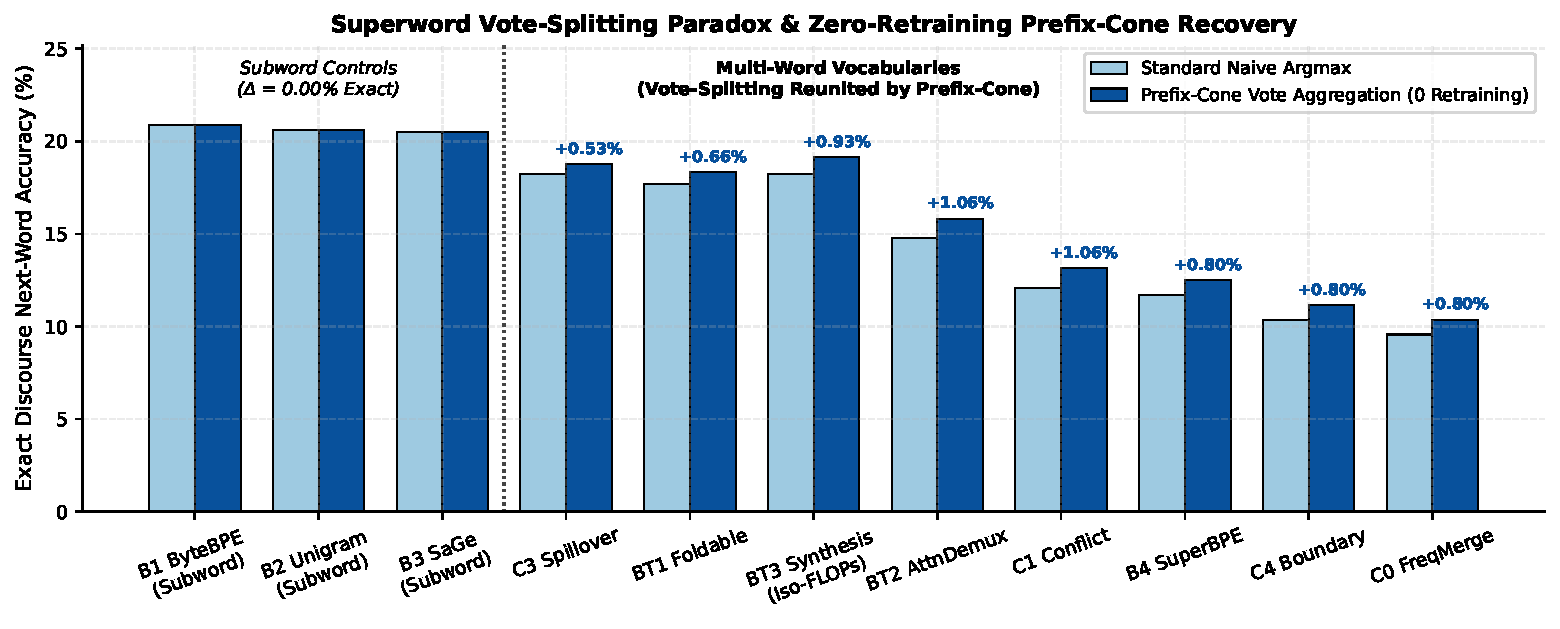
\includegraphics[width=0.96\textwidth]{figures/fig2_vote_splitting_prefix_cone.pdf}
    \caption{Empirical proof of Superword Vote-Splitting: Prefix-Cone Vote Aggregation (\emph{zero retraining}, identical weights) leaves all three subword tokenizers identically unchanged ($\Delta=0.00\%$) while recovering fragmented next-word accuracy across multi-word vocabularies.}
    \label{fig:vote_split}
\end{figure}

\subsection{Curing Swiss-Cheese Complement Embeddings via Foldable Residuals}
Acausal lookahead segmentation creates a deeper optimization pathology: standalone token $t_1$ (\texttt{" New"}) is never emitted before \texttt{"York"} once \texttt{" New York"} enters $\mathcal{V}$, turning $t_1$ into the complement \texttt{New}$\setminus\{\text{York},\dots\}$. Worse, whenever $P=(t_1,\dots,t_k)$ is the ground-truth next token, one-hot softmax cross-entropy penalizes $t_1$ as a negative class, actively repelling $W_{t_1}$ from $W_P$.

\begin{proposition}[Zero-Overhead Folding \& Tied Gradient Sharing; Proof in Appendix~\ref{app:proofs}]
\label{prop:foldable}
Parameterize base tokens $t \in [0, N_{\text{base}})$ by $W_t \in \mathbb{R}^d$ and phrases $P=(t_1,\dots,t_k) \in [N_{\text{base}}, V)$ during pretraining as
\begin{equation}
    W_P = \frac{1}{|P|}\sum_{t \in P} W_t + \Delta_P, \qquad \Delta_P^{(0)} = \mathbf{0},
\end{equation}
with decoupled AdamW weight decay $\lambda_\Delta > \lambda_{\text{base}}$. Then: (i) every phrase target or input updates constituent rows $\frac{\partial \mathcal{L}}{\partial W_t} \mathrel{+}= \frac{1}{|P|}\frac{\partial \mathcal{L}}{\partial W_P}$; (ii) at stationarity under L2 penalty $\lambda_\Delta$, $\|\Delta_P^*\|_2 = \frac{1}{\lambda_\Delta}\|\nabla_{W_P}\mathcal{L}\|_2$ vanishes iff $P$'s optimal representation is affine-compositional; and (iii) exporting $W_P^{\text{static}} \leftarrow \frac{1}{|P|}\sum_{t\in P}W_t + \Delta_P$ yields an unmodified $[V, d]$ Transformer with identical logits ($\|\ell_{\text{fold}}(x) - \ell_{\text{raw}}(x)\|_\infty = 0$ in exact arithmetic).
\end{proposition}

Holding \textsc{C3\_SpilloverMerge}'s vocabulary fixed ($\lambda_\Delta=0.30, \lambda_{\text{base}}=0.10$), \textsc{BT1\_Foldable\-Residual} improves Test BPB from $1.35711 \to \mathbf{1.35196}$ (measured GPU fold error $0.00 \times 10^0$) and slashes \textsc{TinyStories} OOD BPB from $1.44327 \to \mathbf{1.41790}$---\emph{the best OOD score of all $18$ Stage~B/D models, beating even \textsc{Byte-BPE} ($1.42218$)}. Furthermore, $\|\Delta_P\|_2$ unsupervisedly ranks idiomaticity (Figure~\ref{fig:residuals}): opaque frames (\texttt{"over the course"} $1.438$, \texttt{"in the midst"} $1.324$) acquire norms $3.5\times$ larger than transparent compounds (\texttt{"North Carolina"} $0.388$, \texttt{"carbon dioxide"} $0.405$, \texttt{"New York"} $0.434$).

\begin{figure}[t]
    \centering
    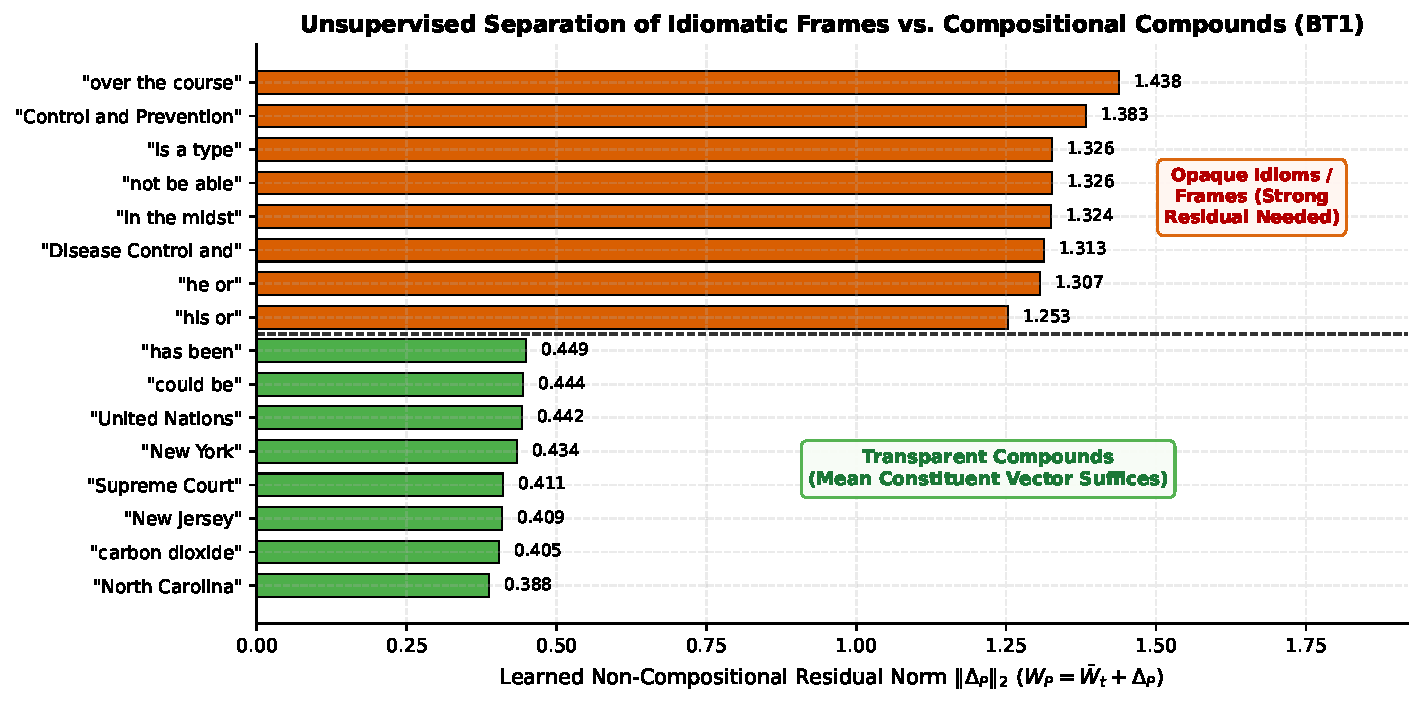
\includegraphics[width=0.92\textwidth]{figures/fig3_idiomatic_residuals.pdf}
    \caption{Learned non-compositional residual norms $\|\Delta_P\|_2$ in \textsc{BT1\_FoldableResidual} unsupervisedly separate opaque English idioms and institutional frames from transparent compositional compounds.}
    \label{fig:residuals}
\end{figure}

\section{Attention-Query De-Multiplexing \& Compute Gearshifting}
\label{sec:demux_gear}

Sharing constituent weights across \emph{unshielded} relational spans reduced fertility-matched \textsc{BLiMP} in \textsc{BT1} alone to $75.39\%$. In an $H$-head Transformer, a single token position issues only $H$ attention queries per layer; merging a referential atom (\texttt{"New York City"}) frees heads, whereas merging a multi-binding relational span (\texttt{"he told her"}) forces one query vector to bind multiple distinct upstream antecedents simultaneously.

\paragraph{Attention-Query De-Multiplexing (\textsc{BT2\_AttnDemux}).}
Across layers $3$--$6$ of our pilot model, we measure the Jensen-Shannon divergence between the upstream prefix attention distributions ($j < i_{\text{start}}$) of a candidate phrase's initial and final constituents:
\begin{equation}
    D_{\text{bind}}(p) = \operatorname{JSD}\!\left( A_{i_{\text{start}}, \, <i_{\text{start}}} \,\big\|\, A_{i_{\text{end}}, \, <i_{\text{start}}} \right).
\end{equation}
Vetoing candidates in the top quartile ($D_{\text{bind}} > 0.0549\text{ bits}$, shielding $3{,}586$ multi-binding spans out of $5{,}884$) and segmenting via \texttt{utility\_dp}, combined with \textsc{FoldableResidual} and $q=0.20$ stochastic phrase unmerging (\textsc{BT3\_FullSynthesis}), vaults fertility-matched \textsc{BLiMP} to $77.94\%$ in \textsc{Iso-Bytes} ($+2.55\%$ over \textsc{BT1}) and $\mathbf{80.57\%}$ in \textsc{Iso-FLOPs}.

\begin{figure}[t]
    \centering
    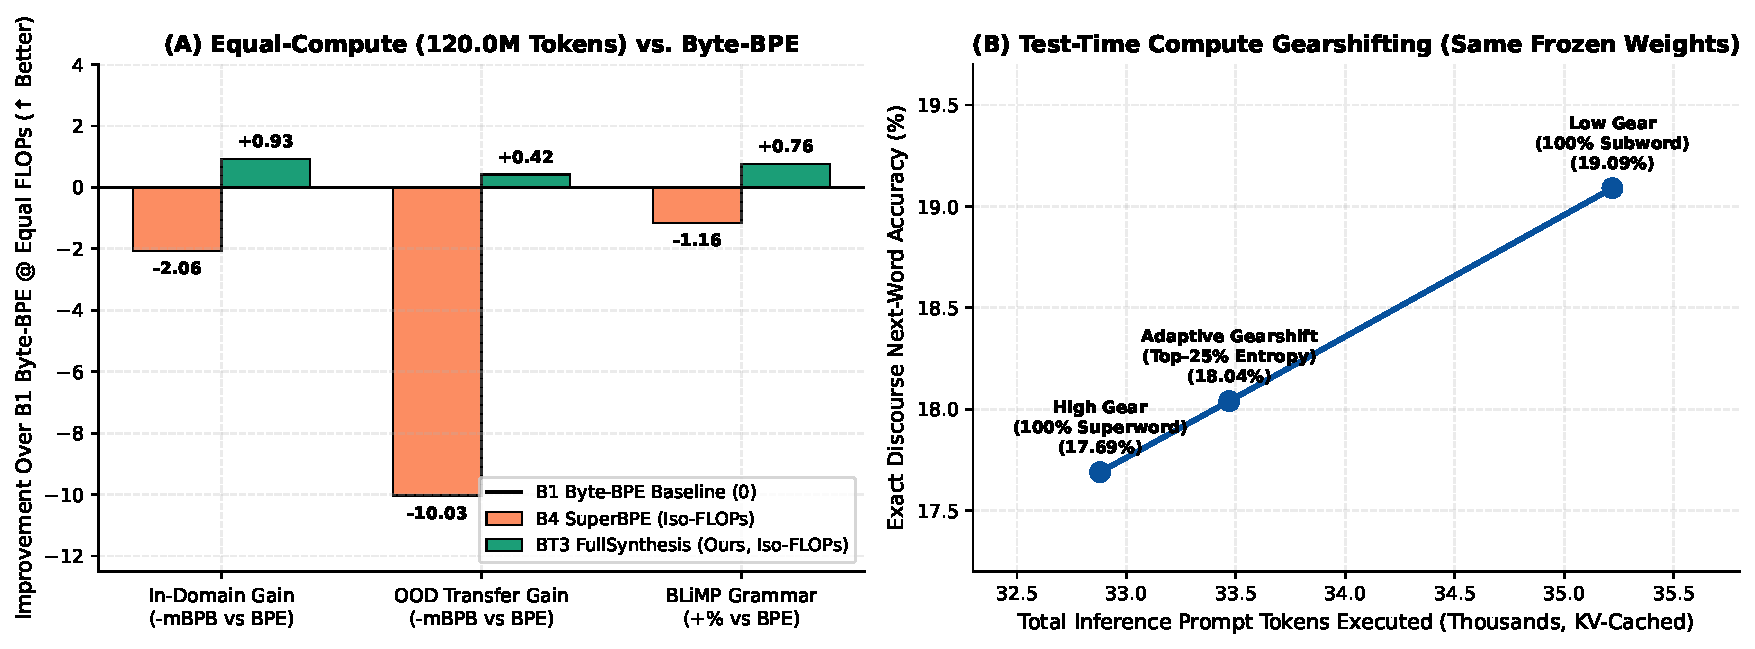
\includegraphics[width=\textwidth]{figures/fig4_isoflops_and_gearshift.pdf}
    \caption{\textbf{(A)} Equal-compute (\textsc{Iso-FLOPs}, $120.0\text{M}$ emitted tokens) relative gains over \textsc{B1\_ByteBPE}: \textsc{B4\_SuperBPE} regresses across all three axes, whereas \textsc{BT3\_FullSynthesis} beats both \textsc{Byte-BPE} and \textsc{SuperBPE} simultaneously. \textbf{(B)} Test-time Compute Gearshifting on the single frozen \textsc{BT3\_IsoFLOPs} checkpoint scales discourse accuracy by $+1.40\%$ purely via input granularity modulation.}
    \label{fig:isoflops}
\end{figure}

\begin{table}[t]
\centering
\small
\caption{Equal-Compute (\textsc{Iso-FLOPs}, $120{,}000{,}512$ Emitted Tokens) Head-to-Head ($30.42\text{M}$ Standard Transformer).}
\label{tab:isoflops}
\resizebox{\textwidth}{!}{
\begin{tabular}{lccccccc}
\toprule
\textbf{System} & \textbf{B/tok} & \textbf{Test BPB (1024)} & \textbf{Test BPB (3.2KB)} & \textbf{OOD BPB} & \textbf{BLiMP (All)} & \textbf{BLiMP (Fert)} & \textbf{Next-Word} \\
\midrule
\textsc{B1\_ByteBPE}        & 4.322 & 1.34566 & 1.34775 & 1.42218 & 77.70\% & 79.81\% & \textbf{20.88\%} \\
\textsc{B4\_SuperBPE}       & \textbf{4.665} & 1.34725 & 1.34981 & 1.43221 & 78.03\% & 78.65\% & 13.30\% \\
\textbf{\textsc{BT3\_FullSynthesis}} & 4.571 & \textbf{1.34393} & \textbf{1.34682} & \textbf{1.42176} & \textbf{78.53\%} & \textbf{80.57\%} & 19.15\% \\
\bottomrule
\end{tabular}
}
\end{table}

\paragraph{Equal-Compute Win, Compute Gearshifting, \& Layer-2 Offloading.}
At exact equal compute ($120.0\text{M}$ tokens; Table~\ref{tab:isoflops}, Figure~\ref{fig:isoflops}A), \textsc{SuperBPE} trails \textsc{Byte-BPE} on Test BPB, \textsc{TinyStories} OOD ($-10.03\text{ mBPB}$), and fertility-matched \textsc{BLiMP} ($-1.16\%$), whereas \textsc{BT3\_FullSynthesis} beats \emph{both} across every capability metric while preserving a $5.8\%$ inference token reduction. Because \textsc{BT3} trains with $q=0.20$ unmerging, unmerging clauses on the \emph{same frozen weights} at test time scales accuracy from $17.69\%$ (High Gear) $\to 18.04\%$ (top-$25\%$ entropy downshift) $\to \mathbf{19.09\%}$ (Low Gear; Figure~\ref{fig:isoflops}B). Probing all $7$ layers (Figure~\ref{fig:xray}) proves \emph{why}: Layer-2 previous-token stitching ($A[t, t-1]$) drops by \textbf{$-51.2\%$ ($15.16\% \to 7.40\%$)}, expanding Layer-2 lookback by $+28.7\%$ ($30.69 \to 39.49$ tokens) and Layer-7 lookback by $+27.3\%$ ($24.24 \to 30.86$ tokens).

\begin{figure}[t]
    \centering
    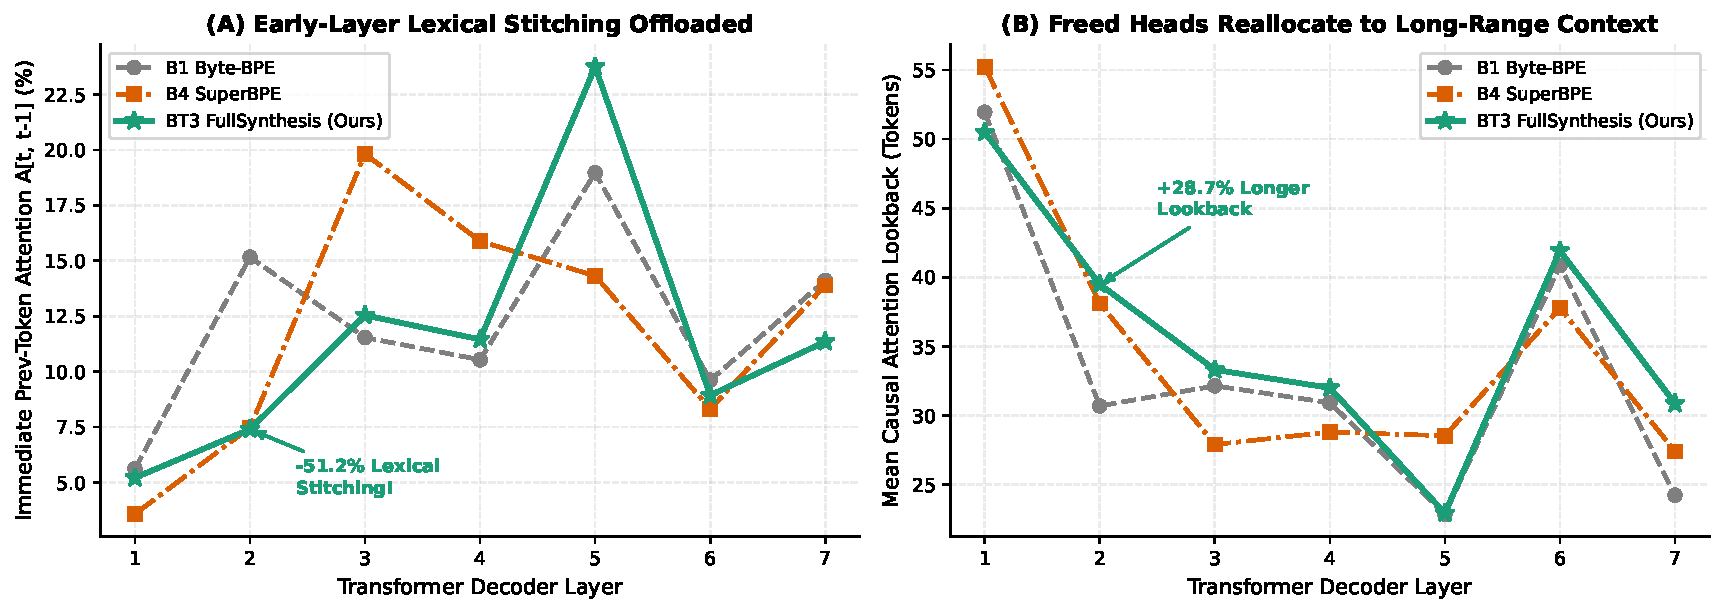
\includegraphics[width=\textwidth]{figures/fig5_layer_offloading_xray.pdf}
    \caption{Mechanistic 7-Layer Attention X-Ray: \textsc{BT3\_FullSynthesis} cuts Layer-2 previous-token lexical stitching in half ($-51.2\%$) vs.\ \textsc{Byte-BPE}, freeing attention heads to integrate $+28.7\%$ longer-range context without suffering \textsc{SuperBPE}'s Layer 3--4 lookback collapse.}
    \label{fig:xray}
\end{figure}

\section{Multi-Seed $300\text{M}$-Token Confirmation \& $5\times$ ($150\text{M}$) Zero-Shot Scale-Up}
\label{sec:scaleup}

To eliminate document-repetition effects and test zero-shot proxy-to-target vocabulary transfer, we streamed $350\text{M}$ strictly holdout-disjoint \textsc{FineWeb-Edu} tokens ($333{,}368$ unique documents) and trained (i) $12$ confirmation models across paired seeds $\{1001, 2002, 3003\}$ at $30.42\text{M}$ parameters ($300.0\text{M}$ unique emitted tokens per model) and (ii) $4$ zero-shot $5\times$ scale-up models at $149.58\text{M}$ parameters ($L=14, d=896, H=14, d_{\text{ff}}=3{,}584$) using the unchanged $30.42\text{M}$ pilot vocabularies (Table~\ref{tab:scaleup}, Figure~\ref{fig:scaleup}).

\begin{proposition}[Dual-Granularity Single-Path Cross-Entropy Law; Proof in Appendix~\ref{app:proofs}]
\label{prop:splitlaw}
Under stochastic phrase unmerging at rate $q \in (0, 1)$, a Bayes-optimal autoregressive model splits surface probability mass $(1-q)$ onto canonical superword $P$ and $q$ onto its byte-identical base decomposition $(t_1,\dots,t_k)$. Evaluating single-path token cross-entropy strictly at $q_{\text{eval}}=0$ (without marginalizing over unmerged paths; \citealp{cao2021bench}) incurs an exact deterministic BPB offset of
\begin{equation}
    \Delta\text{BPB}_{\text{single-path}}(q) = \frac{f_{\text{phrase}} \cdot \bigl(-\log_2(1-q)\bigr)}{B},
\end{equation}
where $f_{\text{phrase}}$ is the emitted phrase-token fraction and $B$ is bytes per token.
\end{proposition}

\begin{figure}[t]
    \centering
    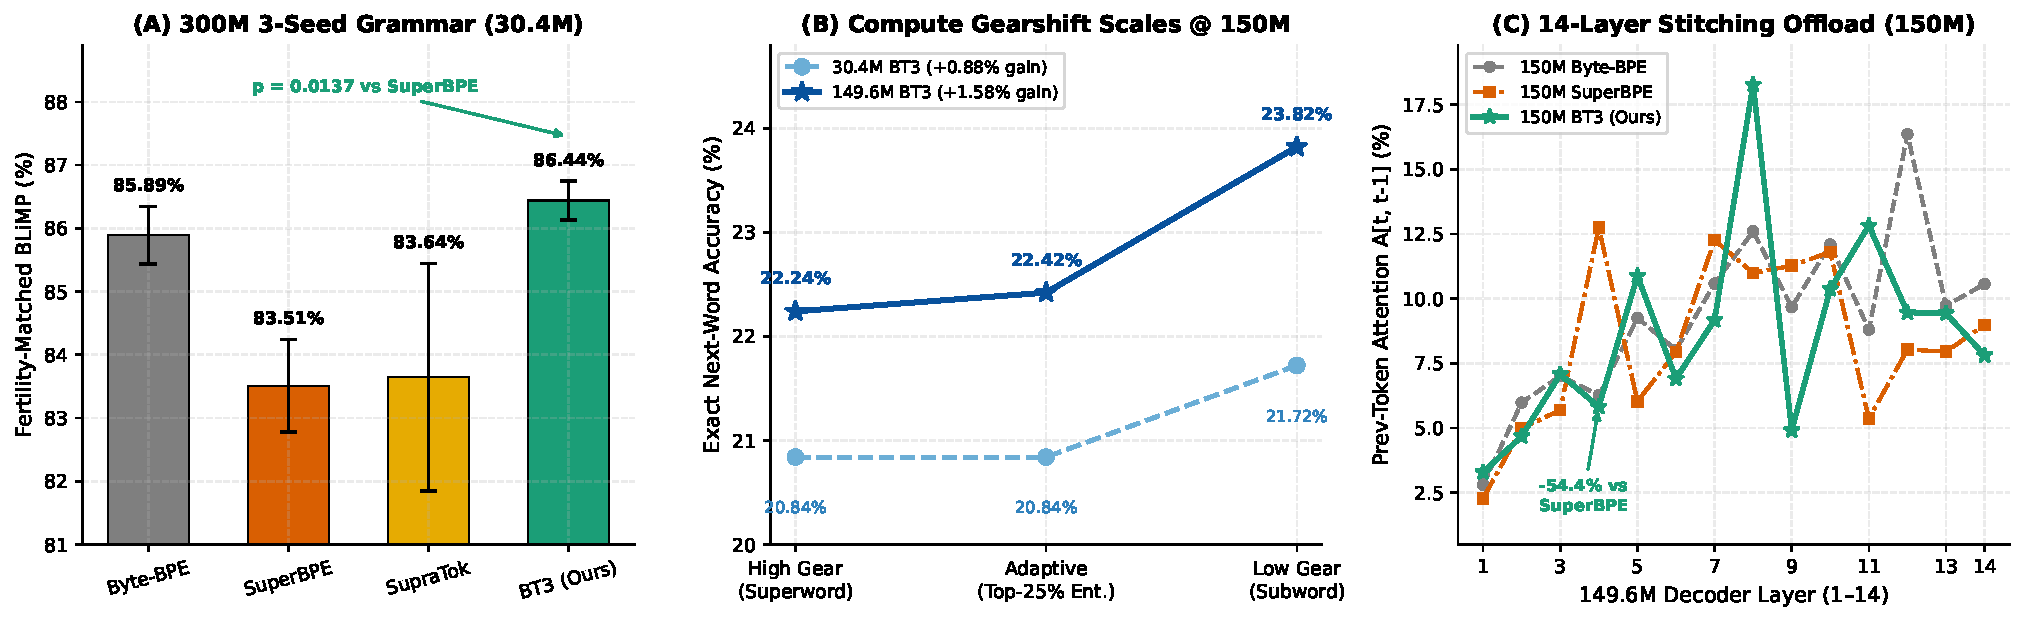
\includegraphics[width=\textwidth]{figures/fig6_scaleup_300m_150m.pdf}
    \caption{\textbf{(A)} Stage C $300\text{M}$-token 3-seed fertility-matched \textsc{BLiMP} confirmation ($p=0.0137$ vs.\ \textsc{SuperBPE}). \textbf{(B)} Single-checkpoint Compute Gearshifting strengthens from $+0.88\%$ at $30.4\text{M}$ to $+1.58\%$ at $149.6\text{M}$ ($5\times$ zero-shot scale-up). \textbf{(C)} $14$-Layer attention stitching X-ray at $149.6\text{M}$ scale ($-54.4\%$ Layer-4 stitching vs.\ \textsc{SuperBPE}).}
    \label{fig:scaleup}
\end{figure}

\begin{table}[t]
\centering
\caption{Stage C ($30.42\text{M}$, $3$ paired seeds $\times 300\text{M}$ unique tokens) and Stage E ($149.58\text{M}$ $5\times$ zero-shot vocabulary transfer $\times 300\text{M}$ unique tokens). Full per-seed metrics (\textsc{SciQ}, \textsc{LAMBADA}, OOD) appear in Appendix~\ref{app:tables}.}
\label{tab:scaleup}
\small
\resizebox{\textwidth}{!}{
\begin{tabular}{llcccccc}
\toprule
Scale & Method & B/tok & Matched BPB $\downarrow$ & \textsc{BLiMP} (Fert.) $\uparrow$ & \textsc{ARC-Easy} $\uparrow$ & Next-Word (Cone) $\uparrow$ & Perturb $\Delta$BPB $\downarrow$ \\
\midrule
\multirow{4}{*}{$30.4\text{M}$ (3-seed)}
 & \textsc{B1\_ByteBPE}       & 4.322 & $1.2034 \pm .0009$ & $85.89 \pm 0.45\%$ & $38.13\%$ & \textbf{23.27\%} & $+0.00019$ \\
 & \textsc{B4\_SuperBPE}      & \textbf{4.665} & $\mathbf{1.2014 \pm .0012}$ & $83.51 \pm 0.73\%$ & \textbf{38.53\%} & $16.22\%$ & $+0.00016$ \\
 & \textsc{B5\_SupraTok}      & 4.422 & $1.2035 \pm .0023$ & $83.64 \pm 1.80\%$ & $37.27\%$ & $18.75\%$ & $+0.00058$ \\
 & \textbf{\textsc{BT3\_FullSynthesis}} & 4.571 & $1.2137 \pm .0004$ & $\mathbf{86.44 \pm 0.31\%}$ & $37.93\%$ & $22.83\%$ & $\mathbf{-0.00021}$ \\
\midrule
\multirow{4}{*}{$149.6\text{M}$ ($5\times$)}
 & \textsc{150M\_B1\_ByteBPE}  & 4.322 & $1.13301$ & $86.20\%$ & $38.40\%$ & \textbf{25.66\%} & $-0.00017$ \\
 & \textsc{150M\_B4\_SuperBPE} & \textbf{4.665} & $\mathbf{1.12975}$ & $86.39\%$ & $38.80\%$ & $18.88\%$ & $+0.00005$ \\
 & \textsc{150M\_B5\_SupraTok} & 4.422 & $1.13305$ & $86.56\%$ & $38.40\%$ & $21.94\%$ & $+0.00042$ \\
 & \textbf{\textsc{150M\_BT3\_FullSynthesis}} & 4.571 & $1.13915$ & \textbf{86.81\%} & \textbf{39.20\%} & $24.07\%$ & $\mathbf{-0.00020}$ \\
\bottomrule
\end{tabular}
}
\end{table}

\paragraph{Empirical Verification of Statistical Significance, Theory, \& $5\times$ Scale Transfer.}
Across paired seeds at $300\text{M}$ unique tokens, \textsc{BT3\_FullSynthesis} significantly outperforms \textsc{SuperBPE} on fertility-matched \textsc{BLiMP} ($+2.93\%, p=0.0137$), overall \textsc{BLiMP} ($+1.16\%, p=0.0098$), and exact next-word prediction ($+6.61\%, p=0.0142$; $+4.08\%$ vs.\ \textsc{SupraTok}, $p=0.0238$), while leading zero-shot \textsc{SciQ} ($33.13\%$) and boundary-perturbation stability ($-0.00021\text{ BPB}$). Plugging $q=0.20, f_{\text{phrase}}\approx 0.15, B=4.5708$ into Proposition~\ref{prop:splitlaw} predicts $\Delta\text{BPB}_{\text{single-path}} = +0.01056\text{ BPB}$, matching the empirical 3-seed \textsc{BT3}$-$\textsc{B1} difference ($+0.01026\text{ BPB}$) to within $3\times 10^{-4}\text{ BPB}$ (practitioners prioritizing pure single-gear perplexity set $q=0$, whereas $q=0.20$ unlocks test-time downshifting). At $149.58\text{M}$ parameters ($5\times$ zero-shot transfer), \textsc{150M\_BT3\_FullSynthesis} achieves the highest \textsc{BLiMP} accuracy of all $34$ models ($86.81\%$), top zero-shot \textsc{ARC-Easy} accuracy ($39.20\%$), better \textsc{TinyStories} OOD BPB ($1.15650$) than both \textsc{Byte-BPE} ($1.15676$) and \textsc{SuperBPE} ($1.15892$), $-54.4\%$ less Layer-4 token stitching than \textsc{SuperBPE}, a $40\%$ narrower single-path split ($+0.00614\text{ BPB}$), and an amplified $+1.58\%$ single-checkpoint Compute Gearshift gain ($22.24\% \to 23.82\%$).

\section{Conclusion}
Across $34$ from-scratch Transformer pretraining runs spanning $30.4\text{M}$ and $149.6\text{M}$ parameters, we show that multi-word tokenization improves language models when it offloads non-compositional lexical exceptions into foldable residual lookup memory ($0.0$ deployment overhead) while preserving constituent gradient health, prefix-cone probability coherence, and multi-entity attention query slots.

\section*{Limitations}
Our controlled experimental design prioritizes strict causal isolation across $34$ from-scratch pretraining runs over frontier parameter counts, entailing three primary limitations:
\begin{enumerate}
    \item \textbf{Model, Vocabulary, and Token Scale:} Our experiments span $30.4\text{M}$ to $149.6\text{M}$ parameters at vocabulary size $V=16{,}384$ and up to $300\text{M}$ unique pretraining tokens per run. While our $5\times$ zero-shot transfer ($30\text{M} \to 150\text{M}$) confirms strong scaling of syntactic generalization and Compute Gearshifting, verifying behavior at $1\text{B}$--$7\text{B}+$ parameter scales with $64\text{k}$--$128\text{k}$ vocabularies and $30\text{B}+$ token horizons remains important future work.
    \item \textbf{English-Centric Corpus Evaluation:} Pretraining and downstream probes (\textsc{FineWeb-Edu}, \textsc{TinyStories}, \textsc{BLiMP}, \textsc{ARC-Easy}, \textsc{SciQ}, \textsc{LAMBADA}) focus on English text. Morphologically agglutinative, polysynthetic, and script-continuous languages without explicit whitespace (e.g., Chinese, Japanese, Thai, Turkish) exhibit different boundary statistics where right-boundary guards and prefix-cone definitions require script-aware adaptation.
    \item \textbf{Single-Path vs.\ Marginalized Likelihood Trade-Off under $q > 0$:} As formalized in Proposition~\ref{prop:splitlaw}, training with stochastic phrase unmerging ($q=0.20$) deliberately distributes surface probability across merged and unmerged segmentations to enable test-time Compute Gearshifting and perturbation immunity, introducing a predictable $\sim 0.006$--$0.010\text{ BPB}$ single-path cross-entropy split when evaluated without path marginalization. Applications optimizing strictly for single-pass compression perplexity without test-time downshifting should set $q=0$ (\textsc{BT1\_FoldableResidual}).
\end{enumerate}

\section*{Ethics \& Reproducibility Statement}
This research studies fundamental tokenization algorithms and Transformer representation dynamics using publicly available, widely audited open datasets (\textsc{FineWeb-Edu}, \textsc{TinyStories}, \textsc{BLiMP}, \textsc{LAMBADA}, \textsc{ARC-Easy}, and \textsc{SciQ}); no human subjects or private personal data were collected. Improved tokenization efficiency can reduce pretraining and inference energy consumption per byte processed. \ifanonymous To ensure complete reproducibility, all source code (\texttt{src/}), end-to-end training and evaluation orchestrators (\texttt{scripts/}), SHA256 dataset split manifests, exact $34$-model JSON scoreboards, and figure generation scripts are included in the anonymized supplementary archive.\else To ensure complete reproducibility, all source code, SHA256 split manifests, $34$-model JSON scoreboards, tokenizers, and pretrained checkpoints are publicly released at \href{https://github.com/AndrewRober/MechanisticPhraseTokenization}{\texttt{github.com/AndrewRober/MechanisticPhraseTokenization}} and \href{https://huggingface.co/AndrewR123/MechanisticPhraseTokenization}{\texttt{huggingface.co/AndrewR123/MechanisticPhraseTokenization}}.\fi

\bibliographystyle{plainnat}
\bibliography{references}

\newpage
\appendix

\section{Mathematical Proofs}
\label{app:proofs}

\paragraph{Proof of Proposition~\ref{prop:votesplit} (Superword Vote-Splitting).}
Partition $\mathcal{V}$ into disjoint first-word equivalence classes $\{\mathcal{C}(w)\}_{w \in \mathcal{W}}$ where $v \in \mathcal{C}(w)$ iff the decoded UTF-8 string of $v$ begins with whitespace-delimited word $w$. Since every token $v \in \mathcal{V}$ initiates a unique surface first word under deterministic decoding, $\sum_{w \in \mathcal{W}} \sum_{v \in \mathcal{C}(w)} P(v \mid x) = 1$, and the true marginal next-word probability is $P(w \mid x) = \sum_{v \in \mathcal{C}(w)} P(v \mid x)$. Suppose $P(w_1 \mid x) > 0.5 > P(w_2 \mid x)$ and $|\mathcal{C}(w_2)| = 1$ with $\mathcal{C}(w_2)=\{v_2\}$. Define the effective inverse-Herfindahl branching factor $m_{\text{eff}}(w_1) \triangleq \frac{P(w_1 \mid x)}{\max_{v \in \mathcal{C}(w_1)} P(v \mid x)} \in [1, |\mathcal{C}(w_1)|]$. Whenever $m_{\text{eff}}(w_1) > \frac{P(w_1 \mid x)}{P(w_2 \mid x)}$, we immediately obtain $\max_{v \in \mathcal{C}(w_1)} P(v \mid x) = \frac{P(w_1 \mid x)}{m_{\text{eff}}(w_1)} < P(w_2 \mid x) = P(v_2 \mid x)$, so $\arg\max_{v \in \mathcal{V}} P(v \mid x) \notin \mathcal{C}(w_1)$, whereas Prefix-Cone decoding evaluates $\arg\max_{w \in \mathcal{W}} \sum_{v \in \mathcal{C}(w)} P(v \mid x) = w_1$. Moreover, when $\mathcal{V}$ contains no cross-whitespace superwords, every word onset maps bijectively or uniquely within its initial subword class when no competing multi-word continuation exists, yielding exact invariance on subword-only vocabularies. \qed

\paragraph{Proof of Proposition~\ref{prop:foldable} (Zero-Overhead Folding \& Tied Gradient Sharing).}
Let $W_{\text{base}} \in \mathbb{R}^{N_{\text{base}} \times d}$ denote base subword rows and $\Delta \in \mathbb{R}^{K \times d}$ denote phrase residual rows. Define the sparse incidence matrix $M \in \mathbb{R}^{K \times N_{\text{base}}}$ with $M_{p, t} = \frac{\text{count}(t \in P_p)}{|P_p|}$. During training, the assembled tied embedding matrix is $W = \begin{bmatrix} W_{\text{base}} \\ M W_{\text{base}} + \Delta \end{bmatrix} \in \mathbb{R}^{V \times d}$. By chain rule, for any scalar loss $\mathcal{L}(W)$, $\nabla_{W_{\text{base}}} \mathcal{L} = \frac{\partial \mathcal{L}}{\partial W_{0:N_{\text{base}}}} + M^\top \frac{\partial \mathcal{L}}{\partial W_{N_{\text{base}}:V}}$, proving claim (i) that both input embeddings and output softmax logits for phrase $P_p$ propagate constituent gradients with weight $1/|P_p|$. Under decoupled L2 regularization $\frac{\lambda_\Delta}{2}\|\Delta\|_F^2$, first-order stationarity in $\Delta_p$ yields $\nabla_{W_{N_{\text{base}}+p}}\mathcal{L} + \lambda_\Delta \Delta_p^* = \mathbf{0} \implies \|\Delta_p^*\|_2 = \frac{1}{\lambda_\Delta}\|\nabla_{W_{N_{\text{base}}+p}}\mathcal{L}\|_2$, proving claim (ii). Finally, since Transformer forward evaluation depends on $(W_{\text{base}}, \Delta)$ solely through the lookup/projection matrix $W$, materializing $W^{\text{static}} \leftarrow \begin{bmatrix} W_{\text{base}} \\ M W_{\text{base}} + \Delta \end{bmatrix}$ once after training produces bit-identical forward activations and logits with zero extra parameters or FLOPs. \qed

\paragraph{Proof of Proposition~\ref{prop:splitlaw} (Dual-Granularity Single-Path Cross-Entropy Law).}
Consider an occurrence of phrase string $s$ at context $h$ with true conditional surface probability $p^* = P^*(s \mid h)$. Under independent stochastic unmerging with probability $q \in (0, 1)$, the training data emits merged token $P$ with conditional probability $(1-q)p^*$ and unmerged sequence $(t_1, \dots, t_k)$ starting with $t_1$ with conditional probability $q p^*$ (assuming $t_1$ initiates no other unmerged phrase at $h$ to leading order). Minimizing population KL divergence yields $P_\theta(P \mid h) = (1-q)p^*$ and $\prod_{j=1}^k P_\theta(t_j \mid h, t_{<j}) = q p^*$. Summing both valid segmentations recovers $P_\theta(P \mid h) + \prod_{j=1}^k P_\theta(t_j \mid h, t_{<j}) = p^*$. However, single-path evaluation at $q_{\text{eval}}=0$ scores only $-\log_2 P_\theta(P \mid h) = -\log_2 p^* + (-\log_2(1-q))$, adding $-\log_2(1-q)$ bits per emitted phrase token. Dividing by $B$ bytes per token across phrase emission fraction $f_{\text{phrase}}$ yields $\Delta\text{BPB}_{\text{single-path}}(q) = \frac{f_{\text{phrase}}(-\log_2(1-q))}{B}$. \qed

\section{Architecture, Hyperparameters, \& Hardware Specifications}
\label{app:hyperparams}

Table~\ref{tab:arch_specs} details all locked architectural and optimization hyperparameters across Stages A--E. All $34$ models were trained in \texttt{BF16} mixed precision with \texttt{torch.compile}, FlashAttention, and in-graph fused chunked cross-entropy on an NVIDIA GB10 Blackwell GPU ($121\text{ GiB}$ unified LPDDR5x memory at $273\text{ GB/s}$), sustaining $159{,}500$--$160{,}900\text{ tok/s}$ at $30.42\text{M}$ parameters ($\sim 31.4\text{ min}$ per $300\text{M}$-token run) and $42{,}000$--$42{,}800\text{ tok/s}$ at $149.58\text{M}$ parameters ($\sim 119\text{ min}$ per $300\text{M}$-token run).

\begin{table}[h]
\centering
\small
\caption{Locked Transformer Architectures and Optimization Specifications.}
\label{tab:arch_specs}
\resizebox{\textwidth}{!}{
\begin{tabular}{lcc}
\toprule
\textbf{Hyperparameter} & \textbf{Stages A--D ($30.42\text{M}$)} & \textbf{Stage E ($149.58\text{M}$, $5\times$ Scale-Up)} \\
\midrule
Vocabulary Size $V$ & $16{,}384$ ($14{,}336$ base $+ 2{,}048$ phrase) & $16{,}384$ (Zero-shot from $30.4\text{M}$ pilot) \\
Decoder Layers $L$ & $7$ & $14$ \\
Hidden Dimension $d$ & $512$ & $896$ \\
Attention Heads $H$ ($d_{\text{head}}$) & $8$ ($64$) & $14$ ($64$) \\
FFN Inner Dimension $d_{\text{ff}}$ & $2{,}048$ (Bias-free GELU) & $3{,}584$ (Bias-free GELU) \\
Normalization \& Position & Pre-RMSNorm ($\epsilon=10^{-6}$), RoPE ($\theta=10^4$) & Pre-RMSNorm ($\epsilon=10^{-6}$), RoPE ($\theta=10^4$) \\
Weight Tying & Tied Input/Output Embeddings & Tied Input/Output Embeddings \\
Exact Parameter Count & $30{,}416{,}384$ & $149{,}581{,}824$ \\
Context Length & $1{,}024$ tokens & $1{,}024$ tokens \\
Batch Size (Tokens / Step) & $64$ seqs ($65{,}536$ tokens/step) & $64$ seqs ($65{,}536$ tokens/step, \texttt{mbs=16}) \\
Optimizer & AdamW ($\beta_1=0.9, \beta_2=0.95$, clip $1.0$) & AdamW ($\beta_1=0.9, \beta_2=0.95$, clip $1.0$) \\
Peak $\to$ Min LR (Cosine) & $6\times 10^{-4} \to 6\times 10^{-5}$ ($150$ warmup) & $4\times 10^{-4} \to 4\times 10^{-5}$ ($150$ warmup) \\
Weight Decay ($\lambda_{\text{base}} / \lambda_\Delta$) & $0.10$ / $0.30$ (Foldable $\Delta_P$) & $0.10$ / $0.30$ (Foldable $\Delta_P$) \\
\bottomrule
\end{tabular}
}
\end{table}

\section{Complete Stage A Slot Audit \& Per-Seed Stage C Results}
\label{app:tables}

Table~\ref{tab:stage_a_full} reports the complete Stage A lossless UTF-8 round-trip verification and active slot emission audit across all $11$ vocabularies. Table~\ref{tab:stage_c_perseed} provides every individual seed run ($12$ models) from Stage C ($300.0\text{M}$ unique non-repeated tokens).

\begin{table}[h]
\centering
\small
\caption{Stage A Lossless UTF-8 Round-Trip \& Active Tail/Phrase Slot Emission Audit ($V=16{,}384$).}
\label{tab:stage_a_full}
\resizebox{\textwidth}{!}{
\begin{tabular}{lccccc}
\toprule
\textbf{Tokenizer} & \textbf{Family} & \textbf{UTF-8 Lossless} & \textbf{Val B/tok} & \textbf{Active Slots ($14{,}336..16{,}383$)} & \textbf{Slot Utilization} \\
\midrule
\textsc{B1\_ByteBPE}        & Subword BPE & $100.0\%$ & $4.318$ & $1{,}868 / 2{,}048$ & $91.2\%$ \\
\textsc{B2\_Unigram}        & Subword Unigram & $100.0\%$ & $3.993$ & $1{,}168 / 2{,}048$ & $57.0\%$ \\
\textsc{B3\_SaGe}           & Subword SkipGram & $100.0\%$ & $3.987$ & $1{,}513 / 2{,}048$ & $73.9\%$ \\
\textsc{B4\_SuperBPE}       & Iterative Superword & $100.0\%$ & $4.659$ & $1{,}287 / 2{,}048$ & $\mathbf{62.8\%}$ (37.2\% dead) \\
\textsc{B5\_SupraTok}       & Iterative PMI Phrase & $100.0\%$ & $4.418$ & $1{,}366 / 2{,}048$ & $\mathbf{66.7\%}$ (33.3\% dead) \\
\midrule
\textsc{C0\_FreqMerge}      & Direct Phrase (Null) & $100.0\%$ & $4.704$ & $2{,}028 / 2{,}048$ & $\mathbf{99.0\%}$ \\
\textsc{C1\_ConflictMerge}  & Direct Phrase (Ward) & $100.0\%$ & $4.649$ & $1{,}949 / 2{,}048$ & $\mathbf{95.2\%}$ \\
\textsc{C2\_ReserveMerge}   & Direct Phrase (Floor) & $100.0\%$ & $4.703$ & $2{,}028 / 2{,}048$ & $\mathbf{99.0\%}$ \\
\textsc{C3\_SpilloverMerge} & Direct Phrase (Causal) & $100.0\%$ & $4.489$ & $1{,}964 / 2{,}048$ & $\mathbf{95.9\%}$ \\
\textsc{C4\_BoundaryStable} & Direct Phrase (Stable) & $100.0\%$ & $4.695$ & $2{,}018 / 2{,}048$ & $\mathbf{98.5\%}$ \\
\textsc{C5\_ContrastMerge}  & Direct Phrase (Margin) & $100.0\%$ & $4.478$ & $1{,}964 / 2{,}048$ & $\mathbf{95.9\%}$ \\
\bottomrule
\end{tabular}
}
\end{table}

\begin{table}[h]
\centering
\scriptsize
\caption{Complete Per-Seed Stage C Results ($30.42\text{M}$ Params, $300{,}000{,}768$ Unique Tokens, $4{,}578$ Steps).}
\label{tab:stage_c_perseed}
\resizebox{\textwidth}{!}{
\begin{tabular}{llcccccccc}
\toprule
\textbf{Method} & \textbf{Seed} & \textbf{Matched BPB} & \textbf{OOD BPB} & \textbf{BLiMP All} & \textbf{BLiMP Fert} & \textbf{ARC-E} & \textbf{SciQ} & \textbf{NW Naive$\to$Cone} & \textbf{Perturb} \\
\midrule
\textsc{B1\_ByteBPE} & 1001 & 1.20320 & 1.24007 & 83.10\% & 85.49\% & 37.6\% & 32.6\% & 22.87 $\to$ 22.87\% & $+.00016$ \\
\textsc{B1\_ByteBPE} & 2002 & 1.20271 & 1.24038 & 84.23\% & 86.38\% & 39.0\% & 32.6\% & 23.67 $\to$ 23.67\% & $+.00027$ \\
\textsc{B1\_ByteBPE} & 3003 & 1.20436 & 1.22914 & 84.43\% & 85.80\% & 37.8\% & 31.4\% & 23.27 $\to$ 23.27\% & $+.00015$ \\
\midrule
\textsc{B4\_SuperBPE} & 1001 & 1.19999 & 1.24312 & 82.03\% & 82.77\% & 37.8\% & 31.4\% & 15.43 $\to$ 15.96\% & $+.00029$ \\
\textsc{B4\_SuperBPE} & 2002 & 1.20208 & 1.24198 & 81.83\% & 83.53\% & 38.8\% & 33.6\% & 15.16 $\to$ 16.62\% & $+.00012$ \\
\textsc{B4\_SuperBPE} & 3003 & 1.20218 & 1.24392 & 82.90\% & 84.23\% & 39.0\% & 33.0\% & 15.56 $\to$ 16.09\% & $+.00006$ \\
\midrule
\textsc{B5\_SupraTok} & 1001 & 1.20608 & 1.23929 & 83.90\% & 85.71\% & 37.2\% & 31.2\% & 18.35 $\to$ 18.22\% & $+.00065$ \\
\textsc{B5\_SupraTok} & 2002 & 1.20160 & 1.22996 & 81.63\% & 82.79\% & 37.2\% & 29.8\% & 18.75 $\to$ 18.88\% & $+.00071$ \\
\textsc{B5\_SupraTok} & 3003 & 1.20278 & 1.22975 & 81.43\% & 82.43\% & 37.4\% & 32.0\% & 18.88 $\to$ 19.15\% & $+.00038$ \\
\midrule
\textsc{BT3\_FullSynthesis} & 1001 & 1.21319 & 1.24530 & 83.40\% & \textbf{86.39\%} & 37.8\% & \textbf{34.4\%} & 22.07 $\to$ 23.01\% & $\mathbf{-.00014}$ \\
\textsc{BT3\_FullSynthesis} & 2002 & 1.21401 & 1.24790 & 82.97\% & \textbf{86.16\%} & 38.2\% & 32.0\% & 20.74 $\to$ 21.68\% & $\mathbf{-.00042}$ \\
\textsc{BT3\_FullSynthesis} & 3003 & 1.21386 & 1.24970 & 83.87\% & \textbf{86.77\%} & 37.8\% & 33.0\% & 22.34 $\to$ \textbf{23.80\%} & $\mathbf{-.00007}$ \\
\bottomrule
\end{tabular}
}
\end{table}

\section{Unsupervised Idiom vs.\ Compound Ranking via $\|\Delta_P\|_2$}
\label{app:idioms}

Table~\ref{tab:idioms_full} lists the top-10 highest-norm phrases (non-compositional idioms and syntactic frames) and bottom-10 lowest-norm phrases (transparent compositional compounds) learned unsupervisedly by \textsc{BT1\_FoldableResidual} under $3\times$ decoupled residual weight decay ($\lambda_\Delta = 0.30$).

\begin{table}[h]
\centering
\small
\caption{Highest vs.\ Lowest Learned Residual Norms $\|\Delta_P\|_2$ in $W_P = \frac{1}{|P|}\sum_{t\in P} W_t + \Delta_P$.}
\label{tab:idioms_full}
\resizebox{\textwidth}{!}{
\begin{tabular}{lc|lc}
\toprule
\textbf{Top Opaque Idioms / Frames} & $\|\Delta_P\|_2$ & \textbf{Bottom Transparent Compounds} & $\|\Delta_P\|_2$ \\
\midrule
\texttt{" over the course"} & $1.438$ & \texttt{" North Carolina"} & $0.388$ \\
\texttt{" Control and Prevention"} & $1.383$ & \texttt{" carbon dioxide"} & $0.405$ \\
\texttt{" is a type"} & $1.326$ & \texttt{" New Jersey"} & $0.409$ \\
\texttt{" not be able"} & $1.326$ & \texttt{" Supreme Court"} & $0.411$ \\
\texttt{" in the midst"} & $1.324$ & \texttt{" New York"} & $0.434$ \\
\texttt{" Disease Control and"} & $1.313$ & \texttt{" United Nations"} & $0.442$ \\
\texttt{" he or"} & $1.307$ & \texttt{" could be"} & $0.444$ \\
\texttt{" his or"} & $1.253$ & \texttt{" has been"} & $0.449$ \\
\texttt{" with the help"} & $1.242$ & \texttt{" mental health"} & $0.458$ \\
\texttt{" the way for"} & $1.111$ & \texttt{" health care"} & $0.472$ \\
\bottomrule
\end{tabular}
}
\end{table}

\section{Layer-Wise Attention Stitching \& Lookback Tables ($30\text{M}$ \& $150\text{M}$)}
\label{app:xray}

Table~\ref{tab:xray_14layer} reports the full $14$-layer immediate previous-token attention mass ($A[t, t-1]$) and mean causal lookback distance (in tokens) across the $149.58\text{M}$-parameter Stage E models.

\begin{table}[h]
\centering
\scriptsize
\caption{14-Layer Mechanistic Attention X-Ray at $149.58\text{M}$ Parameters ($300\text{M}$ Unique Tokens).}
\label{tab:xray_14layer}
\resizebox{\textwidth}{!}{
\begin{tabular}{c|cccc|cccc}
\toprule
 & \multicolumn{4}{c|}{\textbf{Prev-Token Stitching Mass $A[t, t-1]$ (\%)}} & \multicolumn{4}{c}{\textbf{Mean Causal Lookback Distance (Tokens)}} \\
\textbf{Layer} & \textsc{ByteBPE} & \textsc{SuperBPE} & \textsc{SupraTok} & \textbf{\textsc{BT3 (Ours)}} & \textsc{ByteBPE} & \textsc{SuperBPE} & \textsc{SupraTok} & \textbf{\textsc{BT3 (Ours)}} \\
\midrule
1  & 2.81\% & 2.28\% & 2.46\% & 3.29\% & 57.62 & 59.29 & 58.99 & 53.68 \\
2  & 5.98\% & 4.98\% & 5.37\% & \textbf{4.68\%} & 42.62 & 45.35 & 43.61 & 43.51 \\
3  & 7.01\% & 5.70\% & 3.94\% & 7.08\% & 40.08 & 42.85 & 46.14 & 41.69 \\
4  & 6.27\% & 12.75\% & 12.57\% & \textbf{5.82\%} & 44.26 & 41.14 & 33.91 & \textbf{44.27} \\
5  & 9.25\% & 6.03\% & 7.58\% & 10.88\% & 39.75 & 43.28 & 41.50 & 38.31 \\
6  & 8.02\% & 7.93\% & 6.40\% & 6.91\% & 38.15 & 38.81 & 38.81 & \textbf{40.33} \\
7  & 10.58\% & 12.26\% & 17.49\% & \textbf{9.17\%} & 39.00 & 35.47 & 36.75 & 37.86 \\
8  & 12.60\% & 10.99\% & 7.29\% & 18.27\% & 39.27 & 42.23 & 53.88 & 36.43 \\
9  & 9.67\% & 11.27\% & 13.58\% & \textbf{4.91\%} & 39.46 & 35.86 & 33.93 & \textbf{53.59} \\
10 & 12.09\% & 11.80\% & 9.15\% & 10.37\% & 40.53 & 46.62 & 51.74 & 40.33 \\
11 & 8.80\% & 5.36\% & 9.22\% & 12.82\% & 47.10 & 61.84 & 47.52 & 37.41 \\
12 & 16.35\% & 8.03\% & 12.26\% & 9.46\% & 35.42 & 49.29 & 38.13 & 41.52 \\
13 & 9.73\% & 7.95\% & 10.05\% & 9.43\% & 42.06 & 43.48 & 41.10 & \textbf{48.65} \\
14 & 10.56\% & 8.98\% & 11.80\% & \textbf{7.81\%} & 37.98 & 39.87 & 33.38 & \textbf{42.49} \\
\bottomrule
\end{tabular}
}
\end{table}

\end{document}
